%%%%%%%% ICML 2019 EXAMPLE LATEX SUBMISSION FILE %%%%%%%%%%%%%%%%%

\documentclass{article}

% Recommended, but optional, packages for figures and better typesetting:
\usepackage{microtype}
\usepackage{graphicx}
\usepackage{subfigure}
\usepackage{booktabs} % for professional tables

% hyperref makes hyperlinks in the resulting PDF.
% If your build breaks (sometimes temporarily if a hyperlink spans a page)
% please comment out the following usepackage line and replace
% \usepackage{icml2019} with \usepackage[nohyperref]{icml2019} above.
\usepackage{hyperref}

% Attempt to make hyperref and algorithmic work together better:
\newcommand{\theHalgorithm}{\arabic{algorithm}}

% Use the following line for the initial blind version submitted for review:
\usepackage[accepted]{icml2020}

% Highlight contents with \hl{...}
\usepackage{soul}

% If accepted, instead use the following line for the camera-ready submission:
%\usepackage[accepted]{icml2019}

% The \icmltitle you define below is probably too long as a header.
% Therefore, a short form for the running title is supplied here:
\icmltitlerunning{Practical Deep Learning Approach for Intraday Futures Trading}

\begin{document}

\twocolumn[
\icmltitle{Practical Deep Learning Approach for Intraday Futures Trading}

% It is OKAY to include author information, even for blind
% submissions: the style file will automatically remove it for you
% unless you've provided the [accepted] option to the icml2019
% package.

% List of affiliations: The first argument should be a (short)
% identifier you will use later to specify author affiliations
% Academic affiliations should list Department, University, City, Region, Country
% Industry affiliations should list Company, City, Region, Country

% You can specify symbols, otherwise they are numbered in order.
% Ideally, you should not use this facility. Affiliations will be numbered
% in order of appearance and this is the preferred way.
\icmlsetsymbol{equal}{*}

\begin{icmlauthorlist}
\icmlauthor{Yuyuan Cui}{cu}
\icmlauthor{Ziyan Wang}{cu}
\end{icmlauthorlist}

\icmlaffiliation{cu}{Columbia University, New York, USA}

\icmlcorrespondingauthor{Yuyuan Cui}{yc2968@columbia.edu}
\icmlcorrespondingauthor{Ziyan Wang}{zw2569@columbia.edu}

% You may provide any keywords that you
% find helpful for describing your paper; these are used to populate
% the "keywords" metadata in the PDF but will not be shown in the document
\icmlkeywords{Deep Learning, Reinforcement Learning, Trading Strategy}

\vskip 0.3in
]

% this must go after the closing bracket ] following \twocolumn[ ...

% This command actually creates the footnote in the first column
% listing the affiliations and the copyright notice.
% The command takes one argument, which is text to display at the start of the footnote.
% The \icmlEqualContribution command is standard text for equal contribution.
% Remove it (just {}) if you do not need this facility.

%\printAffiliationsAndNotice{}  % leave blank if no need to mention equal contribution
%\printAffiliationsAndNotice{\icmlEqualContribution} % otherwise use the standard text.

\begin{abstract}
This paper provides the modeling approach and preliminary results for using deep learning and reinforcement learning for developing systematic futures trading strategies in intraday timeframe.
\end{abstract}

\section{Introduction}
\label{intro}

Deep learning has been a popular topic in quantitative financial trading. However, few studies have focused on applying deep learning approach to intraday and tick-level data for trading. As tick-level data provides a much larger dataset for training than daily data, and that various order placement types provide more options for action, there is plenty of opportunities to use complicated deep learning architecture for both prediction and strategy formulation. In this paper, we develop two independent models for China’s IH futures intraday trading based on tick-level high frequency data. The first model is an LSTM model that focuses on short-term price change prediction only. We will then combine the model prediction with a manually formulated simple trading strategy with take-profit and stop-loss thresholds to make trading decisions. The second model is a deep reinforcement learning model whose action space includes buy and sell decisions and hence will output an entire trading strategy on its own. On top of that, we will set up a passive market-making strategy as benchmark. By comparing their performance, we can evaluate the applicability of reinforcement learning and deep learning in intraday futures trading with different degrees of human experience intervention.

\section{Related Work}

Xiong, Liu, Zhong, Yang and Walid (2018) used deep reinforcement learning to obtain optimal strategy based on daily return data of 30 selected stocks\cite{xiong2018practical}. Xiao Zhong and David Enke (2019) used DNNs to predict daily ETF return based on 60 financial and economic features. Sezer, Ozbayoglua, and Dogdub (2017) used DNNs for optimizing technical indicators for daily stock trading and independently trained models for each of selected 30 stocks\cite{SEZER2017473}.

\section{Problem Statement}

The objective is to design deep learning models that maximize trading profit for IH futures\footnote{IH future is based on SSE 50 Index, one of the most popular index futures traded in CFFEX} based on tick-level high frequency data. We will build two individual models in this project. The first one focuses on short-term price movement prediction only and we will manually formulate a simple trading strategy based on its predictions. The second model uses deep reinforcement learning and will output trading actions on its own. In addition, we will set up a passive market-making strategy as benchmark\footnote{enter and exit a position on best bid and offer}. By comparing their performance, we can evaluate the applicability of reinforcement learning and deep learning in intraday futures trading with various degrees of human experience intervention.

\section{Methods}

\subsection{LSTM for Mid Price Change Prediction}

Due to the sequential nature of time series order book tick data, we apply LSTM and linear regression in our deep learning model for mid price change prediction problem. We define LSTM with 1 hidden layer, 256 hidden features and 90 samples with 90 seconds interval. Then we process the final output of LSTM with a two-stage linear regression to get the predicted price change\ref{fig:lstm}.

\begin{figure}[h]
	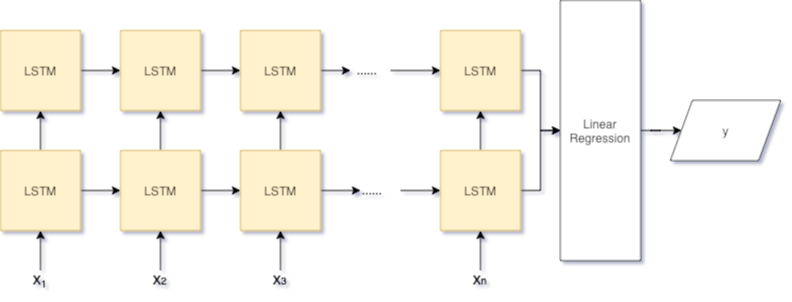
\includegraphics[width=\linewidth]{lstm.png}
	\caption{In each training, the LSTM part ingests 90 samples of data and produce the final output to linear regression. The price change is predicted by the linear regression}
	\label{fig:lstm}
\end{figure}

The reason why we use price change as our prediction target as opposed to return is that there is no fundamental change in price scale (e.g. due to share split or drastic volatility regime shift) during the entire training and testing data sample, and that our trading horizon is constrained to be intraday. We train the model using hl{stochastic gradient decent algorithm}.

Where $x_t$ is the vector of following features as of time $t$:

\begin{itemize}
\setlength\itemsep{0.1em}
\item ${mid\_lag}_T$ ($T=1,5,10,30$): difference between current IH mid price and its mid price $T$ seconds before
\item ${mid\_vol}_T$ ($T=30$): IH mid price volatility in the past $T$ seconds
\item ${spread}_T$ ($T=10,30,60$): IH mid weighted price spread in $T$ seconds
\item ${signed\_tick}_T$ ($T=10,30$): number of up price changes minus number of down price changes in the past $T$ look-back interval
\item ${total\_volume}_T$ ($T=10,30$): total IH trading volume in past $T$ seconds look-back interval
\item ${signed\_volume}_T$ ($T=10, 30$): trade-direction signed IH trading volume in past $T$ look-back interval
\item ${IF\_mid\_lag}_T$ ($T=5,30$): difference between current IF mid price and its mid price $T$ seconds before
\item ${IF\_mid\_vol}_T$ ($T=60$): IF mid price volatility in the past $T$ seconds
\item ${IF\_spread}_T$ ($T=10$): IF mid weighted price spread in $T$ seconds
\item ${IF\_total\_volume}_T$ ($T=5,30$): total IF trading volume in past $T$ seconds look-back interval
\item ${IC\_mid\_lag}_T$ ($T=5,30$): difference between current IC mid price and its mid price $T$ time unit before
\item ${IC\_mid\_vol}_T$ ($T=60$): IC mid price volatility in the past $T$ seconds
\item ${IC\_spread}_T$ ($T=10$): IC mid weighted price spread in $T$ seconds
\item ${IC\_total\_volume}_T$ ($T=5,30$): total IC trading volume in past $T$ seconds look-back interval
\end{itemize}

Compared with previous research that only focus on daily returns as predictive features, we take advantage of the most granular level of tick-by-tick data (with average update frequency of less than one second), and construct a wide range of features that encompass information in order book imbalance, trading volume, trading direction, technical time series patter, and cross-asset returns. The reason why we choose not to include cross-asset trade or book information is because based on out-sample testing, the additional predictive power to that already included in cross-asset price change is not meaningful and hence we prefer a simpler model for robustness consideration.

\subsection{Deep Reinforcement Learning for Intraday Trading}

As a trading strategy’s action space can be conveniently described as either buy, hold or sell (see \ref{fig:rl_strat}), we can train a Deep Q Learning (DQN) model to achieve end-to-end training for a trading model (see the training loop in \ref{fig:rl_loop}). 

\begin{figure}[h]
	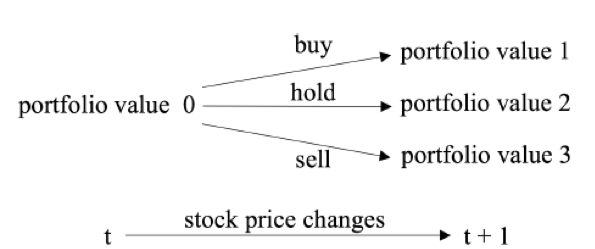
\includegraphics[width=\linewidth]{rl_strat.png}
	\caption{We've defined three actions for Q-learning: buy, hold and sell.}
	\label{fig:rl_strat}
\end{figure}

\begin{figure}[h]
	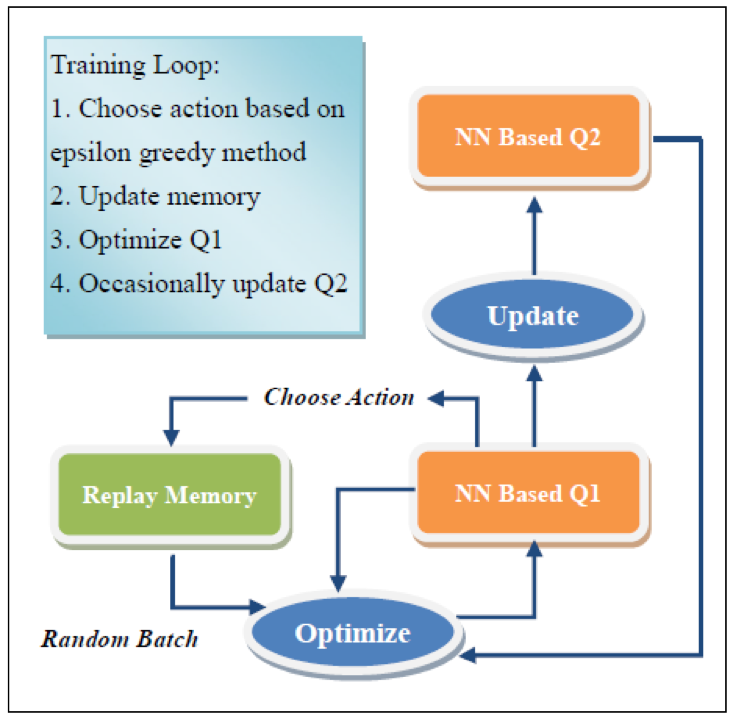
\includegraphics[width=\linewidth]{rl_loop.png}
	\caption{The training Loop for our DQN model}
	\label{fig:rl_loop}
\end{figure}

To characterize the state space, we will use the same features in the LSTM model for comparison purpose. In addition, we add current futures position holding as feature describing the environment. For simplicity, we restrict actions to be either long one additional contract, short one additional contract or no change in position held. As a result, the DNN’s output should be three-dimensional to reflect estimate of value of these three actions. Furthermore, to facilitate calibration, we use market value of position holding 15 minutes since initial setting up a position as “terminal state”. Due to high degree of noise commonly seen in financial data, we choose a Double Q-learning approach to improve robustness and alleviate the risk of overestimating action values. Specifically, we will use the following iterative approach to update the two DNN-based Q(st, at) function estimates, with a cyclic buffer for memory replay. 

\section{Preliminary Results}

\subsection{Data}

The dataset we use is tick data of IH futures (SSE 50 Stock Index Futures), IC futures (CSI 500 Stock Index Futures) and IF (CSI 300 Stock Index Futures) futures tick data in China’s CFFEX exchange in 2018. The data include all book updates and trade events. The morning trading session is 09:30 AM - 11:30 AM local time, while the after session is 01:00 PM – 03:00 PM local time. We treat data in any look-back period prior to session start (e.g. 9:20 AM or 12:30 PM) as NaN but otherwise treat both sessions equally. For each future, we will use front-month contract (contract that expires in the next month). As maximum tick frequency is around 0.5 seconds for all these futures, we regularize all tick data with resample frequency of 0.5 seconds. For missing data, we fill last traded price, bid/offer price and size with most recent valid value; and fill traded volume with 0. For back-testing setup, we always close all positions whenever a trading session ends. The model training period is 1/1/2018 to 8/31/2018, and the testing period is 11/1/2018 to 12/31/2018.

\subsection{Model Performance}

We evaluate the LSTM model using mean-squared error (MSE) of predicted compared with actual mid price change in the testing dataset. Model performance is compared with OLS using same set of features as benchmark\ref{tab:perf}.

\begin{table}[h]
	\begin{center}
		\begin{tabular}{ | c | c | c | } 
			\hline
			& In-sample MSE & Out-sample MSE \\ 
			\hline
			LSTM &  0.56 & 0.75 \\ 
			OLS & 1.7 & 2.2 \\
			\hline
		\end{tabular}
	\end{center}
	\caption{Performance comparison between our LSTM model and the OLS model (benchmark)} \label{tab:perf}
\end{table}

Next, we compare the performance of a simple trading strategy guided by the LSTM with the benchmark passive market-making strategy. The LSTM-based strategy places bid order only when the model predicts the price will move up by more than 0.2, places ask order only when the model predicts the price will move down by more than 0.2, and doesn’t not place any order otherwise. The benchmark passive strategy, however, always places both a bid and an offer order. We restrict both strategy to hold a maximum of one contract at a time. The cumulative profit-and-loss (PnL) plot is as figure\ref{fig:lstm_pnl}:

As our next step, we will evaluate deep reinforcement network model through back-testing performance and comparing it with benchmark passive market-making strategy.

\begin{figure}[h]
  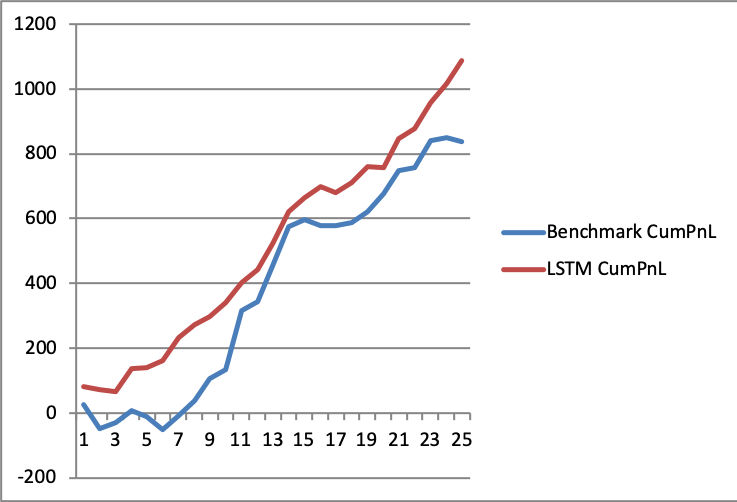
\includegraphics[width=\linewidth]{lstm_pnl.png}
  \caption{Trading PnL of the strategy based on our LSTM model and the benchmark strategy}
  \label{fig:lstm_pnl}
\end{figure}

\subsection{Analysis}

The LSTM model has greater flexibility in capturing both the sequential dependency and complex inter-feature interaction of the high dimensional feature time series. As a result, both in-sample and out-sample MSE are significantly lower than OLS. The market making strategy guided by the model also outperforms purely passive (uninformed) trading strategy. The benchmark strategy trades more frequently and often suffer from adverse selection due to its passive mechanism, and can experience large drawdown even in an intraday horizon. In comparison, the LSTM-based model is more cautious in entering into positions and only trades when it has confidence in predicted direction.

\subsection{Project Repository}
\href{https://github.com/louiswang01/deep-learning-for-futures-trading}{https://github.com/louiswang01/deep-learning-for-futures-trading}

% In the unusual situation where you want a paper to appear in the
% references without citing it in the main text, use \nocite
%\pagebreak
\bibliographystyle{icml2020}
\bibliography{milestone}


\end{document}


% This document was modified from the file originally made available by
% Pat Langley and Andrea Danyluk for ICML-2K. This version was created
% by Iain Murray in 2018, and modified by Alexandre Bouchard in
% 2019. Previous contributors include Dan Roy, Lise Getoor and Tobias
% Scheffer, which was slightly modified from the 2010 version by
% Thorsten Joachims & Johannes Fuernkranz, slightly modified from the
% 2009 version by Kiri Wagstaff and Sam Roweis's 2008 version, which is
% slightly modified from Prasad Tadepalli's 2007 version which is a
% lightly changed version of the previous year's version by Andrew
% Moore, which was in turn edited from those of Kristian Kersting and
% Codrina Lauth. Alex Smola contributed to the algorithmic style files.
